\documentclass[tikz, border=10pt]{standalone}
\usetikzlibrary{calc}

\begin{document}
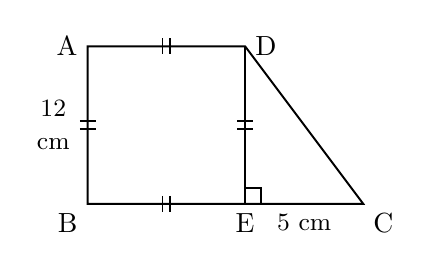
\begin{tikzpicture}[line width=0.7pt]
    % স্থানাঙ্ক নির্ধারণ (Coordinates)
    \coordinate (B) at (0,0);
    \coordinate (A) at (0,2);
    \coordinate (D) at (2,2);
    \coordinate (E) at (2,0);
    \coordinate (C) at (3.5,0);

    % জ্যামিতিক আকার অঙ্কন (Drawing shapes)
    \draw (A) -- (D) -- (C) -- (B) -- cycle; % বাইরের সীমানা
    \draw (D) -- (E); % DE লম্ব

    % সমকোণ চিহ্ন (Right angle at E)
    \draw (2,0.2) -- (2.2,0.2) -- (2.2,0);

    % টিক মার্ক (Tick marks for equal sides)
    % AB বাহুর মাঝে
    \draw (-0.1, 1.05) -- (0.1, 1.05);
    \draw (-0.1, 0.95) -- (0.1, 0.95);
    % AD বাহুর মাঝে
    \draw (0.95, 2.1) -- (0.95, 1.9);
    \draw (1.05, 2.1) -- (1.05, 1.9);
    % BE বাহুর মাঝে
    \draw (0.95, 0.1) -- (0.95, -0.1);
    \draw (1.05, 0.1) -- (1.05, -0.1);
    % DE বাহুর মাঝে
    \draw (1.9, 1.05) -- (2.1, 1.05);
    \draw (1.9, 0.95) -- (2.1, 0.95);

    % লেবেল এবং পরিমাপ (Labels and Measurements)
    \node[left] at (A) {A};
    \node[below left] at (B) {B};
    \node[below] at (E) {E};
    \node[below right] at (C) {C};
    \node[right] at (D) {D};

    \node[left, align=center] at (-0.1, 1) {\small 12 \\ \small cm};
    \node[below] at (2.75, 0) {\small 5 cm};

\end{tikzpicture}
\end{document}